%%%%%%%%%%%%%%%%%%%%%%%%%%%%%%%%%%%%%%%%%%%%%%%%%%%%%%%%%%%%%%%%%%
%%%%%%%%%%%%%%%%%%%%%%%%%%%%%%%%%%%%%%%%%%%%%%%%%%%%%%%%%%%%%%%%%%

\subsection{Introduction}
Le système d'exploitation développé est exécuté sur une architecture \acrshort{IA-32}
aussi appelée i386. Ceci veut dire que la mémoire est adressée sur 32 bits.
$2^{32}=4Go$, donc la mémoire physique (\acrshort{ram}) a une taille totale de
4Go dans notre système d'exploitation. Lorsqu'une tache est exécutée, elle est chargée
en mémoire et est définie par la paire base et limite. La base est son adresse physique
dans la \acrshort{ram} et la limite est sa taille. La figure \ref{ex_base_limit}
donne un exemple d'adressage de plusieurs processus.\cite{ref42}

\begin{figure}[!h]
  \centering
  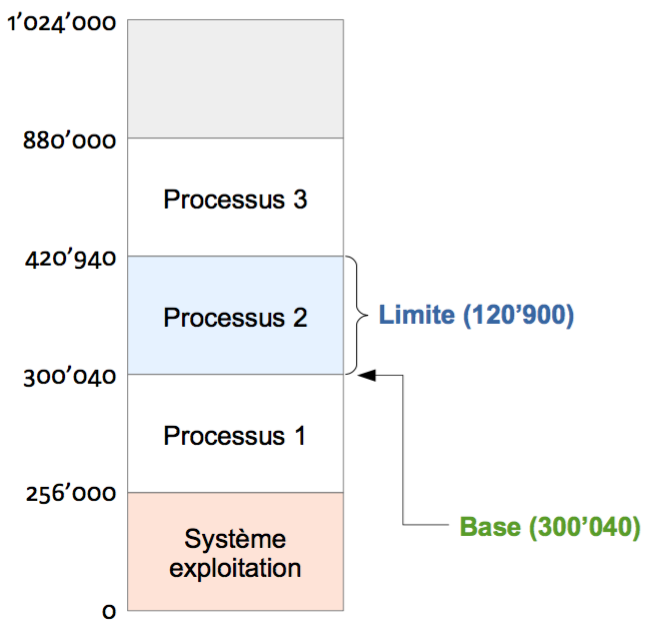
\includegraphics[scale=0.5]{images/ex_base_limit.png}
  \caption{Exemple d'adressage mémoire}
  \label{ex_base_limit}
\end{figure}

Une tache possède son propre espace d'adressage dit virtuel. Pour le processus 1
de la figure \ref{ex_base_limit}, l'adresse $0$ est en fait à l'adresse physique
$300040$. Il y a donc besoin de translater l'adresse virtuelle en adresse physique.
C'est là qu'entre en jeu le \acrshort{mmu} (Memory Mangement Unit). Le \acrshort{mmu}
est un dispositif matériel permettant de faire cette translation d'adresses. A chaque
référencement mémoire, il va convertir l'adresse virtuelle en adresse physique et
regarder si elle ne dépasse pas la limite du processus. Le \acrshort{mmu} permet donc
aussi de protéger la mémoire car il va empêcher toute référence à une zone extérieure
au processus (voir figure \ref{mmu}).\cite{ref42}

\begin{figure}[!h]
  \centering
  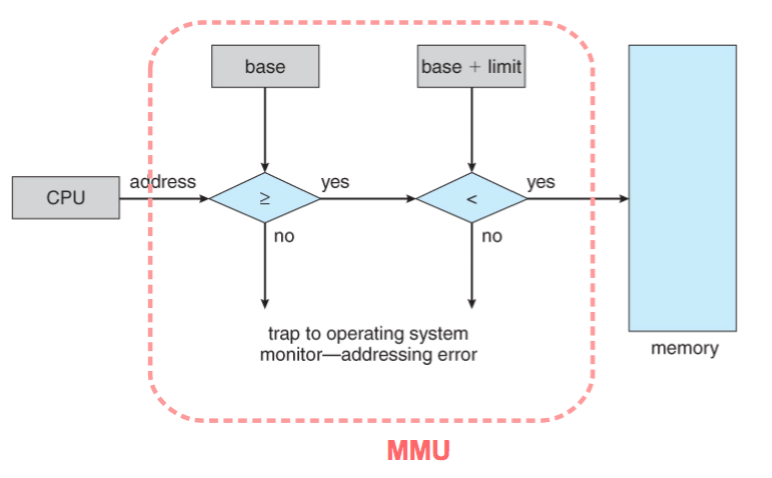
\includegraphics[scale=0.4]{images/mmu.png}
  \caption{Protection mémoire avec un \acrshort{mmu}}
  \label{mmu}
\end{figure}

%%%%%%%%%%%%%%%%%%%%%%%%%%%%%%%%%%%%%%%%%%%%%%%%%%%%%%%%%%%%%%%%%%
%%%%%%%%%%%%%%%%%%%%%%%%%%%%%%%%%%%%%%%%%%%%%%%%%%%%%%%%%%%%%%%%%%

\subsection{\acrshort{gdt}}
Dans une architecture \acrshort{IA-32}, la translation d'adresses se fait à l'aide
de descripteurs définissant des segments de mémoire. Ces descripteurs sont contenus
dans une table de descripteurs. Cette table est la \acrshort{gdt} (Global Descriptor
Table) \cite{ref14}. Chaque descripteur est défini par sa base (son adresse physique),
sa limite (sa taille) et son niveau de privilèges (allant de 0 à 3, le niveau 0 
ayant le plus de privilèges et le niveau 3 le moins). Ci dessous, la figure \ref{gdt}
montre un exemple d'une \acrshort{gdt}.\cite{ref42}

\begin{figure}[!h]
  \centering
  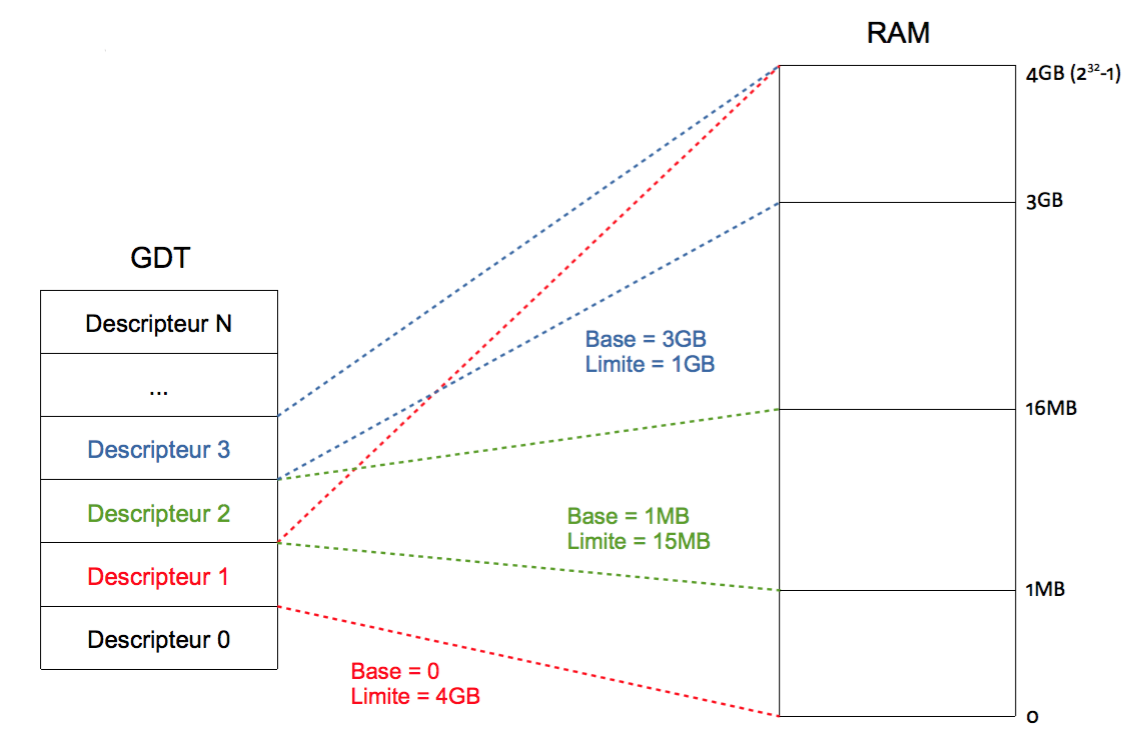
\includegraphics[scale=0.7]{images/gdt.png}
  \caption{Exemple d'une \acrshort{gdt}}
  \label{gdt}
\end{figure}

La \acrshort{gdt} est contenue en mémoire. Chaque entrée (ou descripteur) de
la table de descripteurs sont sur 64 bits et sont définis par la structure de
la figure \ref{gdt_entry}.\cite{ref14}

\begin{figure}[!h]
  \centering
  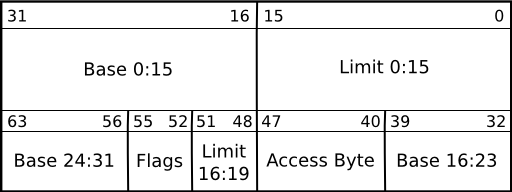
\includegraphics[scale=0.75]{images/gdt_entry.png}
  \caption{Structure d'une entrée dans la \acrshort{gdt}}
  \label{gdt_entry}
\end{figure}

\begin{itemize}[label=\textbullet]
	\item La base est sur 32 bits et est divisée en 3 parties dans une entrée.
    Les bits 16 à 31, 32 à 39 et 56 à 63 contiennent la base
	\item La limite est sur 20 bits et est divisée en 2 parties dans une entrée.
    Les bits 0 à 15 et 48 à 51 contiennent la limite
	\item L'\textit{Access byte} contient des bits de contrôle pour l'accès aux données
    du segment (privilèges, écriture ou lecture, etc...). Il est décrit plus en détail
    dans la figure \ref{gdt_bits}
    \item Les \textit{Flags} sont aussi des bits de contrôle et sont décrits plus
    en détail dans la la figure \ref{gdt_bits}\cite{ref14}
\end{itemize}

\begin{figure}[!h]
  \centering
  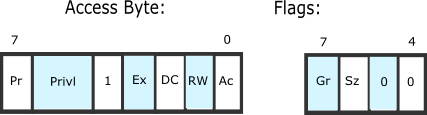
\includegraphics[scale=0.75]{images/gdt_bits.png}
  \caption{\textit{Access byte et Flags}}
  \label{gdt_bits}
\end{figure}

\begin{itemize}[label=\textbullet]
	\item Pr : \textit{Present} bit, doit être à 1 si le segment est valide
	\item Privl : Niveau de privilèges sur deux bits
	\item Ex : \textit{Executable bit}, est à 1 si le segment peut être exécuté
    (par exemple dans un segment de code, ce bit est à 1 alors que dans un segment
    de données, ce bit est à 0)
    \item DC : \textit{Direction bit}
    \item RW : Bit de lecture/ écriture
    \item Ac : \textit{Accessed bit}, ce bit est mis à 1 lorsque le \acrshort{cpu}
    accède à ce segment
    \item Gr : Bit de granularité, à 0 la limite est en octets, à 1 la limite est en blocs
    de 4Ko
    \item Sz : \textit{Size bit}, à 0 le segment est sur 16 bits, à 1 le segment
    est sur 32 bits
\end{itemize}

Par exemple, pour obtenir un segment sur toute la mémoire disponible, il faut mettre
le bit de granularité à 1 (pour avoir une limite en blocs de 4Ko) et mettre la
limite à 0xFFFFF. Une fois la \acrshort{gdt} construite, il faut utiliser l'instruction
\mintinline{text}{lgdt} pour la charger. L'adresse du descripteur de la \acrshort{gdt}
doit être donnée en argument à cette instruction. Le descripteur de \acrshort{gdt}
est défini par la structure 48-bits décrite dans la figure \ref{gdt_descriptor}.\cite{ref14}

\begin{figure}[!h]
  \centering
  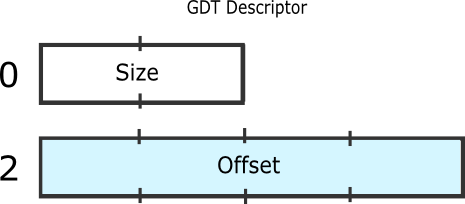
\includegraphics[scale=0.5]{images/gdt_descriptor.png}
  \caption{Descripteur de \acrshort{gdt}}
  \label{gdt_descriptor}
\end{figure}

\begin{itemize}[label=\textbullet]
	\item \textit{Size} est la limite sur 16 bits (c'est à dire la taille de la
    \acrshort{gdt} - 1)
	\item \textit{Offset} est l'adresse physique de la \acrshort{gdt} sur 32 bits
\end{itemize}

\newpage

%%%%%%%%%%%%%%%%%%%%%%%%%%%%%%%%%%%%%%%%%%%%%%%%%%%%%%%%%%%%%%%%%%
%%%%%%%%%%%%%%%%%%%%%%%%%%%%%%%%%%%%%%%%%%%%%%%%%%%%%%%%%%%%%%%%%%

\subsection{Segmentation}
La segmentation est une technique permettant de découper la mémoire en segments
de mémoire logique. Une adresse logique est convertie par le \acrshort{mmu} en
adresse linéaire en utilisant une \acrshort{gdt} ou une \acrshort{ldt}.
Si la pagination (dont on parlera plus tard) est activée, l'adresse linéaire
est convertie en adresse physique. Toute cette mécanique est décrite dans la figure
\ref{addr_translation}. La segmentation permet de faire la convertion d'adresse
logique en adresse linéaire et est obligatoire en mode protégé (32-bits).\cite{ref17}

\begin{figure}[!h]
  \centering
  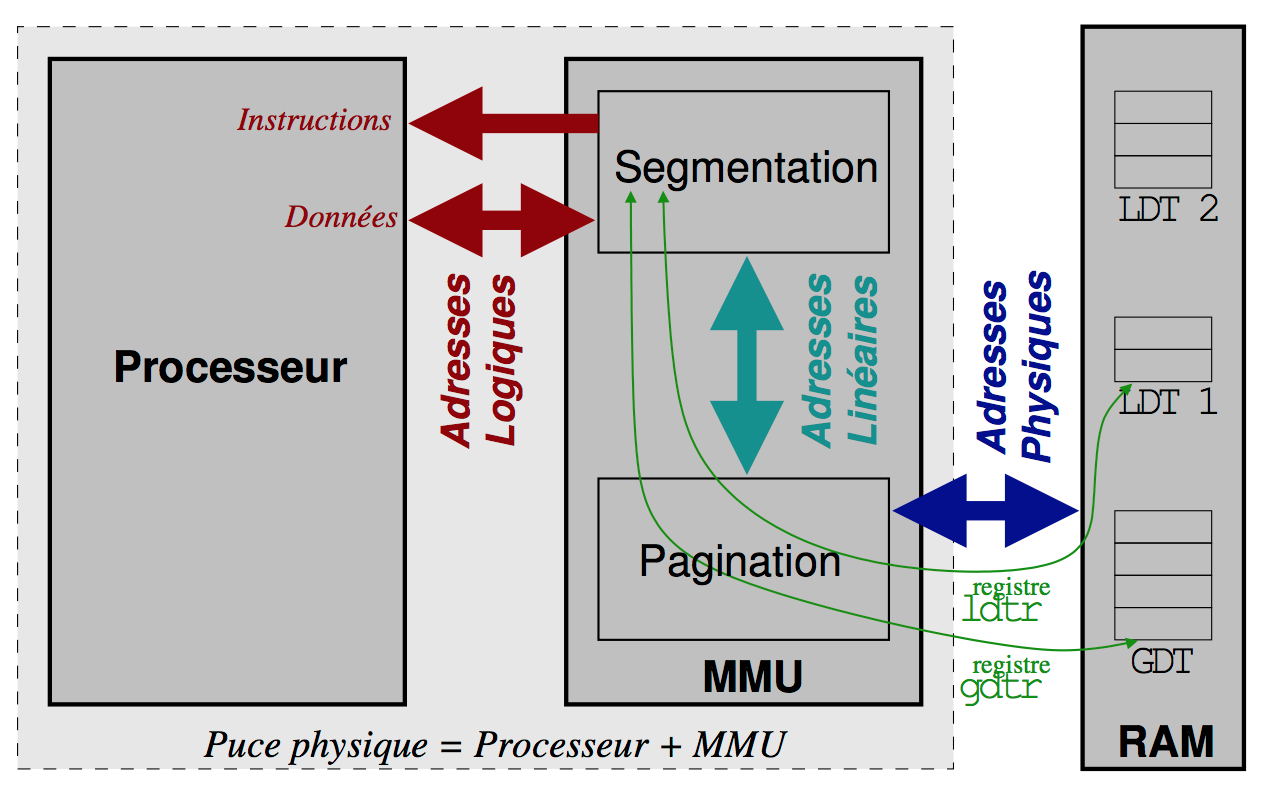
\includegraphics[scale=0.5]{images/addr_translation.png}
  \caption{Translation d'adresse}
  \label{addr_translation}
\end{figure}

La gestion de la segmentation par le \acrshort{cpu} se fait à l'aide de registres
spéciaux nommés registres de segment. Ces registres sont au nombre de 6 et ont
chacun une taille de 16 bits.\cite{ref42,ref18}

\begin{center}
	\scalebox{1}{
		\begin{tabular}{| C{5cm} | C{5cm} | }
			\hline
			Registre & Segment \\ \hline
			CS & \textit{Code Segment} \\ \hline
			DS & \textit{Data Segment} \\ \hline
			SS & \textit{Stack Segment} \\ \hline
			ES & \textit{Extra Segment} \\ \hline
			FS & \multirow{2}{*}{\textit{General Purpose Segments}} \\
            GS & \\ \hline
		\end{tabular}
	}
\end{center}

En mode protégé (32-bits), ces registres doivent pointer sur des descripteurs
de segment de la \acrshort{gdt}. Au minimum les trois premiers registres décrits
doivent être utilisé en mode protégé (CS, DS, et SS). Les opérations adressant le
code (décodage des instructons en mémoire, sauts, etc...) référencent le descripteur
de segment sur lequel pointe le registre CS. Les opérations adressant les données
(adressage de variables ou d'adresses mémoires) référencent le descripteur de segment
sur lequel pointe le registre DS. Les opérations adressant la pile (\mintinline{text}{push}
et \mintinline{text}{pop}) référencent le descripteur de segment sur lequel pointe
le registre SS. \\

Nous avons vu qu'un descripteur de segment fait 64 bits et un registre de segment
fait 16 bits. Ceci est possible car le registre de segment ne va pas contenir
l'integralité d'une entrée dans la \acrshort{gdt} mais un sélecteur de cette entrée.
Un sélecteur a une taille de 16 bits (comme les registres de segment) et contient
l'index du descripteur dans la \acrshort{gdt}, un bit indiquant si l'entrée est
dans la \acrshort{gdt} ou dans la \acrshort{ldt} ainsi que son niveau de privilège
(figure \ref{seg_sel}).\cite{ref42}

\begin{figure}[!h]
  \centering
  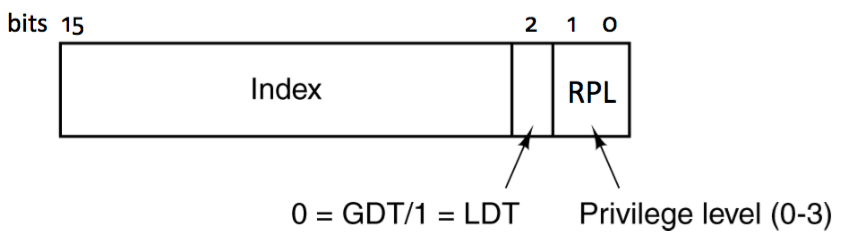
\includegraphics[scale=0.75]{images/seg_sel.png}
  \caption{Structure d'un sélecteur de segment}
  \label{seg_sel}
\end{figure}

Pour récupérer l'index dans la \acrshort{gdt} d'un segment à partir de son descripteur,
il faut donc faire un décallage de 3 bits. Prennons un segment si situant à l'index
2 de la \acrshort{gdt}. Si on veut initialiser le segment de code (registre CS)
avec ce segment, il faut mettre la valeur 16 dans le registre CS ($2 << 3 = 16$). \\

Dans un premier temps, l'\acrshort{os} développé a eu un adressage segmenté de type
\textit{FLAT}, c'est-à-dire que toute la mémoire était accédée de manière linéaire.
Ceci se fait en initialisant trois descripteurs dans la \acrshort{gdt}. Un descripteur
nul à l'index 0 (obligatoire dans touts les modèles de segmentation), un segment
de code couvrant toute la mémoire et un segment de données couvrant aussi toute la mémoire.
Les segments de code et de données adressent donc les mêmes zones de mémoire.
On verra par la suite que d'autres entrées ont été aujoutées à la \acrshort{gdt}
pour la gestion des tâches.

%%%%%%%%%%%%%%%%%%%%%%%%%%%%%%%%%%%%%%%%%%%%%%%%%%%%%%%%%%%%%%%%%%
%%%%%%%%%%%%%%%%%%%%%%%%%%%%%%%%%%%%%%%%%%%%%%%%%%%%%%%%%%%%%%%%%%

\subsection{Pagination}
\subsubsection{Principe général}
La pagination est une autres techinque de gestion de mémoire qui diffère de la
segmentation. Alors que la segmentation permet d'allouer des morceaux de mémoire
de taille variable, la pagination divise la mémoire en blocs de taille fixe appelés
pages (de 4Ko, 2Mo ou 4Mo). De plus, la segmentation est obligatoire dans une
architecture i386 alors que la pagination ne l'est pas\cite{ref16}. Quand une tâche
fait référence à une adresse logique en mémoire, cette adresse est convertie en
adresse linéaire grace au mécanisme de segmentation et c'est le mécanisme de
pagination qui permet de translater cette adresse linéaire en adresse physique
(comme vu précedemment dans la partie sur la segmentation). Quand la
pagination est activée, l'adresse linéaire est divisée en deux parties lorsque
des pages de 4Mo sont utilisées et en trois parties lorsque des pages de 4Ko
sont utilisées. Le \textit{kernel} développé utilise des pages de 4Ko, une adresse
linéaire est donc sous la forme suivante :

\begin{itemize}[label=\textbullet]
	\item 10 bits pour le \textit{directory index}
	\item 10 bits pour le \textit{page index}
    \item 12 bits pour l'\textit{offset}
\end{itemize}

On dit que cette pagination est une pagination à trois niveaux. En général, une
pagination à trois niveaux est utilisée mais il peut exister des systèmes utilisant
plus ou moins de niveaux. Le système d'exploitation doit créer un répertoire de pages
(\textit{Page Directory}) et au moins une table de pages (\textit{Page Table}) pour
chaque tâche. Les répertoires et les tables de pages ont la taille d'une page et sont
composées d'entrées sur 32 bits (4 octets). Une entrée dans un répertoire permet
d'adresser une table de pages et une entrée dans une table permet d'adresser une page.
Dans notre cas, un répertoire permet donc d'adresser 1024 tables et une table
1024 pages ce qui permet bien d'adresser au total 4Go ($1024 \times 1024 \times 4096$).
Une entrée est sur 32 bits mais seulement les 20 bits de poids fort sont utilisés
pour l'adressage car les adresses sont alignées avec 4096 ce qui laisse les 12 bits
de poids faible pour la configuration.\cite{ref21}

\begin{figure}[!h]
  \centering
  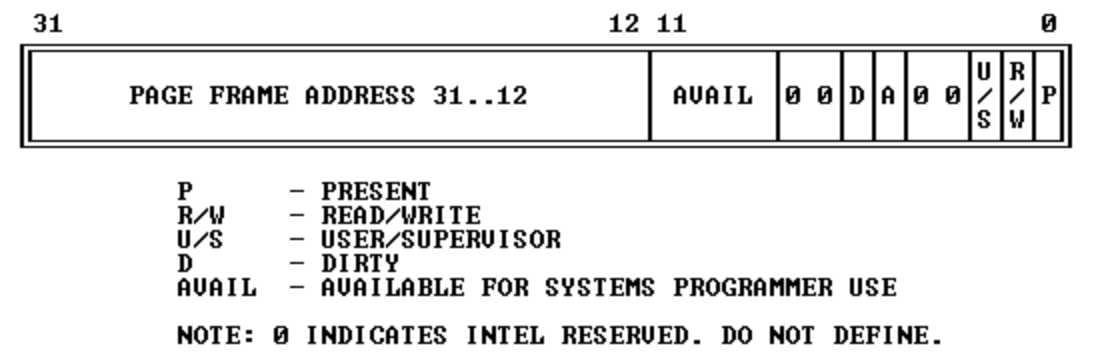
\includegraphics[scale=0.6]{images/page_entry.png}
  \caption{Structure d'une \textit{Page Entry}}
  \label{page_entry}
\end{figure}

Quand une adresse linéaire est lue, le \textit{directory index} permet
de lire la bonne entrée dans le \textit{Page Directory}. Il faut ensuite utiliser
le \textit{page index} pour récupérer la bonne entrée dans la table des pages.
De la même manière que l'entrée dans le répertoire de pages pointait sur une table
des pages, l'entrée dans une table des pages pointe sur une \textit{Page Frame}.
Cette page contient finalement la donnée pointée par l'adresse linéaire, il faut
utiliser l'\textit{offset} pour trouver cette donnée dans la page. La figure \ref{paging3}
résume bien ce mécanisme.\cite{ref66} A noter que le \textit{Page Directory} est
pointé par le registre CR3. A chaque fois qu'un changement de tâche a lieu, le
registre CR3 doit être mis à jour avec le \textit{Page Directory} de la nouvelle
tâche.\cite{ref15}

\begin{figure}[!h]
  \centering
  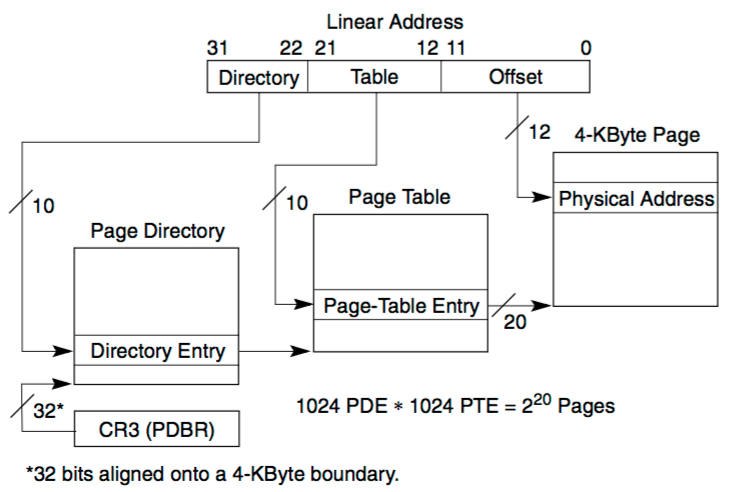
\includegraphics[scale=0.85]{images/paging3.png}
  \caption{Exemple de pagination à 3 niveaux}
  \label{paging3}
\end{figure}

%%%%%%%%%%%%%%%%%%%%%%%%%%%%%%%%%%%%%%%%%%%%%%%%%%%%%%%%%%%%%%%%%%

\subsubsection{Activer la Pagination}
Pour initialiser la pagination sur architecture x86, il faut d'abord construire
un répertoire de pages valide contenant les entrées vers les pages du \textit{kernel}.
Il est obligatoire de commencer par cela car si la pagination est activée et que
le \textit{kernel} n'est pas \textit{mappé} dans le répertoire chargé, une exception
sera levée (\textit{Page Fault}). Par soucis de simplicité pour la suite du développement
de l'\acrshort{os}, le \textit{kernel} va être déplacé au dernier Go de la \acrshort{ram}.
Grace à la pagination, ceci peut se faire assez simplement, il suffit de compléter
le répertoire de pages ainsi que ses tables de pages correctement. Pour rappel,
le \textit{kernel} commence à l'adresse 0x100000 (1Mo) mais il faut aussi rendre
accessible le premier Mo de \acrshort{ram}. Il faut donc déplacer les adresses physiques
allant de 0x0 à la fin du kernel (qui n'est pas fixe). Dans un premier temps, le
\textit{linker} doit être modifié de cette manière :

\begin{minted}[fontsize=\footnotesize,linenos,frame=single,tabsize=4]{c}
SECTIONS {
    /* Low memory Kernel */
    . = 0x00100000;
    .boot ALIGN(4) :        { *(.multiboot) }
    .low_text ALIGN (4K) :  { *(.low_text) }
    .low_data ALIGN (4K) :  { *(.low_data) }
    .low_bss ALIGN (4K) :   { *(.low_bss) }
    /* Higher-half Kernel */
    . += 0xC0000000;
    .stack ALIGN(4) : AT(ADDR(.stack) - 0xC0000000)     { *(.stack) }
    .text ALIGN(4K) : AT(ADDR(.text) - 0xC0000000)      { *(.text*) }
    .rodata ALIGN(4K) : AT(ADDR(.rodata) - 0xC0000000)  { *(.rodata*) }
    .data ALIGN(4K) : AT(ADDR(.data) - 0xC0000000)      { *(.data*) }
    .bss ALIGN(4K) : AT(ADDR(.bss) - 0xC0000000)        { *(COMMON) *(.bss*) }
}
\end{minted}

Ici, le \textit{kernel} est divisé en deux parties. La première est celle qui va
être appelée au démarrage du système et qui va initialiser la pagination. Une fois
la pagination active, le \textit{kernel} va continuer son exécution dans la deuxième
partie qui est située dans le dernier Go de \acrshort{ram}. Nous sommes obligés de
démarrer le \textit{kernel} au début de la mémoire physique car toutes les adresses
sont virtuelles. En réalité, le \textit{kernel} dispose de beaucoup moins (variable
selon la configuration de l'émulateur, ici QEMU). Il n'existe donc pas d'adresse
physique située à 3Go dans la mémoire physique du \textit{kernel} et il est donc
impossible de démarrer le système à cette adresse. Regardons plus en détail de quelle
manière la première partie du \textit{kernel} initialise la pagination. Comme dit
précedemment, un répertoire de pages initial doit être construit. Etant donné que
nous allons exécuter du code dans le premier Go et aussi dans le dernier, le \textit{kernel}
doit être \textit{mappé} dans ces deux zones mémoire en même temps. La première
partie va être adressée linéairement, ce qui veut dire que l'adresse physique
0x0 correspondra à l'adresse virtuelle 0x0 et ainsi de suite jusqu'à la fin du
\textit{kernel}. Cet adressage donne le répertoire de pages shématisé dans la figure
\ref{low_kern_pd}.

\begin{figure}[!h]
  \centering
  \includegraphics[scale=0.65]{images/low_kern_pd.png}
  \caption{Répertoire de pages adressant le \textit{kernel} au début de la \acrshort{ram}}
  \label{low_kern_pd}
\end{figure}

On peut voir ici que la première entrée du répertoire de pages pointe sur une
table de pages adressant le début de la \acrshort{ram}. Chaque entrée est incrémentée
de 4096 (0x1000 en hexadécimal) car une page fait 4096 octets. De plus, les deux
premiers bits de poids faible de chaque page sont à 1 pour indiquer que la page est
active et que l'on peut écrire et lire dedans (voir figure \ref{page_entry}). L'entrée
dans le répertoire de page correspondant au dernier Go (soit 0xC0000000 en hexadécimal)
doit pointer sur une table des pages identique. Pour trouver une entrée dans le
répertoire de pages depuis une adresse il faut faire un décallage à droite de 22
bits sur cette adresse (ce qui est équivalent à diviser par 4096, soit la taille
d'une page, puis de nouveau diviser par 1024, soit le nombre de pages adressées par
une table). Ici, 0xC0000000 $>>$ 22 = 0x300 (768 en décimal). Il faut donc faire
pointer l'entrée 768 du répertoire de pages à une table des pages identique à
celle pointée par l'entrée 0 ce qui donne finalement le répertoire suivant.

\begin{figure}[!h]
  \centering
  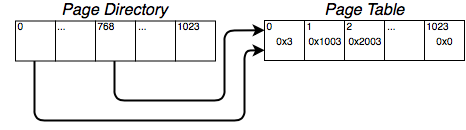
\includegraphics[scale=0.65]{images/high_kern_pd.png}
  \caption{Répertoire de pages adressant le \textit{kernel} à la fin de la \acrshort{ram}}
  \label{high_kern_pd}
\end{figure}

Une fois le répertoire de pages initialisé de cette manière, il ne reste plus
qu'à faire pointer le registre CR3 dessus et activer la pagination en mettant
le bit 31 du registre CR0 à 1. Le code peut ensuite sauter à la partie haute de
la \acrshort{ram} où nous avons déplacé le \textit{kernel}. A partir de là,
tout le code qui sera exécuté sera dans le dernier Go de \acrshort{ram}, il n'y
a donc plus besoin de faire pointer la première entrée du répertoire de pages
sur le table des pages du \textit{kernel} ce qui peut être fait en écrivant 0
dans cette entrée. Le code rust peut finalement être appelé avec la pagination
active.